\chapter{Analysis}
The system must be capable of performing 3D reconstruction based on the eye-in-hand principle, meaning that a stereo camera is mounted at the end-effector of a robot arm. Implementation of the system must be based on the Robot Operating System (ROS) as this is the controller interface for both robot and sensors. The architecture of the system(Figure \ref{fig:block_diagram}) is a closed loop structure based on the Good Old Fashion Artificial Intelligence(GOFAI) environment interaction model \cite{Pfeifer2007a}. In the following each part of the system will be analysed with respect to functionality and responsibilities leading to a formulation of a requirements specification.

\begin{figure}[htb]
	\begin{center}
		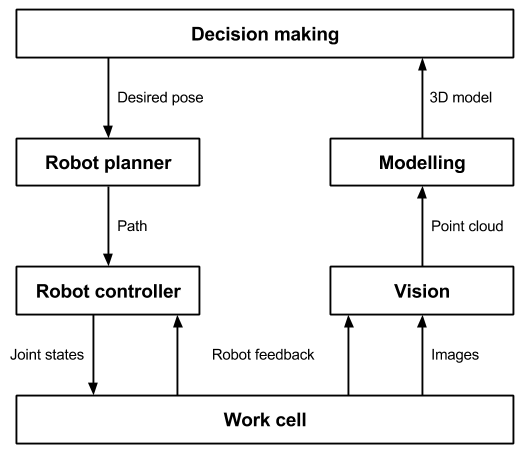
\includegraphics[scale=0.5,trim=0 0 0 0]{graphics/02_analysis/block_diagram.png}%trim=l b r t
		\caption{Block diagram of the eye-in-hand 3D reconstruction system.}
		\label{fig:block_diagram}
	\end{center}
\end{figure}

\subsection{Decision maker}
The decision maker is the highest level of abstraction and authority in the system and is responsible for controlling the task, which in this case means moving the robot arm to the right poses and capture images from the sensor. The task can be broken down to starting the process, choosing a pose, executing the pose, capturing the image and ending the task when there are no more poses needed. Any further work like next best view planning, automatic calibration or other alternative tasks will be implemented in the decision maker and it should therefore be general and easy to expand. In the current application, the desired poses will be generated to capture the object from a number of discrete locations on a sphere subject to distance and viewpoint constraints. The captions must be evenly distributed to cover the entire object. 

\marginnote{Errors...} 


\subsection{Robot planner}
The robot planner is the top level abstraction of the robot arm and takes desired pose in 3D space as input generating a desired path in joint space as output. It is responsible for generating the path between the current pose of the robot and the desired pose. The path is subject to a number of physical constraints and must therefore be generated in steps. The first step is to find a collision free path through the workspace thus requiring a kinematic model of the robot as well as a priori 3D models of robot and work cell. When a suitable path has been found, the path must be optimised for length, clearance and undesired movement. In cases where a collision free path cannot be found, the robot planner must relay this back to the decision maker. Implementations in the robot planner must be robust and therefore make use of some of the widely used open source libraries and ROS stacks should be facilitated. 

\subsection{Robot controller}
The robot controller executes the path and thus handles communication to low level controllers and feedback sensors on the robot. The path is executed in a closed-loop control system and therefore the joint states realising the path must be converted to actuator velocities. This is done by adding a time dimension to the path, subject to joint velocity constraints. The time tessellated path is further blended to meet acceleration and jerk constraints and is finally interpolated and executed in the control loop. Implementations should be robust and therefore make use of some of the many open source libraries and ROS stacks. 

\subsection{Work cell}
The workcell contains a six degrees of freedom RX60 robot arm with a bumblebee stereo camera and a carmine sensor mounted on the end effector(Figure \ref{fig:block_diagram}). The work cell interface is based on a ROS node communicating with the physical robot controller and a node broadcasting data from the camera. Since the RX60 has limited reach, the objects being modelled are hanged from a point over the robot. The a priori model of the work cell contains only the robot arm and simplified bounding boxes representing the immediate surroundings of the robot. 

\marginnote{Image missing}
%\begin{figure}[htb]
%	\begin{center}
%		\includegraphics[scale=0.5,trim=0 0 0 0]{graphics/02_analysis/work_cell.png}%trim=l b r t
%		\caption{The work cell containing RX60 robot mounted with stereo camera.}
%		\label{fig:work_cell}
%	\end{center}
%\end{figure}

\subsection{Vision}
The vision module takes input from the stereo camera mounted on the end effector of the robot and from that generates a 3D point cloud. The images are undistorted and rectified using calibration parameters obtained independently of the system using the ROS calibration node. When the robot is at rest in the desired pose, a signal from the decision maker tells the vision component to capture the two images from the sensor. From the two images a disparity image is formed and by using the obtained projective parameters the point cloud is generated. Implementation should be based on ROS packages and the OpenCV library for image processing.

\subsection{Modelling}
The Modelling part takes point clouds as input and these are transformed to a common frame based on the absolute pose from which they were recorded and a relative pose estimated from matching the points. The combined point cloud is then cropped and filtered to be ready for 3D surface reconstruction. The reconstruction process is performed offline and produces 3D models.

\subsection{Calibration}
The calibration process is responsible for calibrating the system prior to running the task. There are numerous sources of errors in the system, but in a closed-loop system thorough calibration can limit the effects of inaccuracies. Performing a hand-eye calibration can provide the exact transform between camera view and the end-effector, thus in theory removing the need for relative pose estimation in combining the point clouds.

\subsection{Evaluation}
To evaluate the effects of the calibration a series of tests must be made comparing results from the uncalibrated system to results from the calibrated system. Comparison will be made by visual inspection of the produced 3D model. More quantitative measures could be made by using known objects (i.e. objects manufactured from a 3D model) and statistically compare the reconstructed model to the original. However if the difference is not visible to the naked eye, it is not worth doing the calibration. The system should be evaluated using known objects with different levels of detail since this will make it possible to do quantitative evaluation of the system performance if necessary in a future application.

\subsection{Requirements specification}
The above analysis leads to a requirements specification (Table \ref{tab:requirements}) for the combined system.

\begin{table}
	\label{tab:requirements}
	\caption{Requirements specification}
    \begin{tabular}{|l|l|l|}
    \hline
    Block            & Component      & Requirements                                       \\ \noalign{\hrule height 2pt}
    Decision maker   & Pose generator & poses on an equidistant sphere                     \\ \hline
    ~                & ~              & viewpoint at the object                            \\ \hline
    ~                & ~              & evenly distributed                                 \\ \hline
    ~                & State machine  & choose pose                                        \\ \hline
    ~                & ~              & ready for capture signal                           \\ \hline
    ~                & Error handler  & handle impossible pose                             \\ \noalign{\hrule height 2pt}
    Robot planner    & Detector       & detect self collision                              \\ \hline
    ~                & ~              & detect work cell collision                         \\ \hline
    ~                & Planner        & find collision free path                           \\ \hline
    ~                & Optimisation   & optimise path length                               \\ \hline
    ~                & ~              & optimise clearance                                 \\ \hline
    ~                & ~              & remove undesired movement                          \\ \hline
    ~                & Model          & forward kinematics                                 \\ \hline
    ~                & ~              & inverse kinematics                                 \\ \hline
    ~                & ~              & joint limits                                       \\ \noalign{\hrule height 2pt}
    Robot controller & Blender        & tessellation in time                               \\ \hline
    ~                & ~              & handle velocity, acceleration and jerk constraints \\ \hline
    ~                & Control        & get feedback                                       \\ \hline
    ~                & ~              & interpolate path                                   \\ \hline
    ~                & ~              & closed loop control                                \\ \hline
    ~                & Communication  & set joint angles                                   \\ \hline
    ~                & ~              & get joint angles                                   \\ \noalign{\hrule height 2pt}
    Work cell        & Objects        & hang from above the robot                          \\ \hline
    ~                & ~              & known model of objects                             \\ \hline
    ~                & Interface      & ROS based                                          \\ \noalign{\hrule height 2pt}
    Vision           & Camera         & ROS interface                                      \\ \hline
    ~                & ~              & calibration for intrinsic parameters               \\ \hline
    ~                & ~              & calibration for projective parameters              \\ \hline
    ~                & Preprocessor   & undistortion                                       \\ \hline
    ~                & ~              & rectification                                      \\ \hline
    ~                & Controller     & capture images when signaled                       \\ \hline
    ~                & Processor      & generate disparity image                           \\ \hline
    ~                & ~              & generate point cloud                               \\ \noalign{\hrule height 2pt}
    Modelling        & Filtering      & transform points to common frame                   \\ \hline
    ~                & ~              & downsample                                         \\ \hline
    ~                & ~              & combine point clouds                               \\ \hline
    ~                & Reconstruction & generate surface                                   \\ \hline
    \end{tabular}
\end{table}
